% Introduce the chapters contents
% Talk about the Ranking Statistic
% Talk about how we have improved the ranking statistic
% Talk about the offline ranking statistic
% Talk about which parts of the ranking statistic we can use/take
% Talk about how each part of the ranking statistic works

In this chapter I will talk about the improvements made to the PyCBC Live search's ranking statistic which has enabled an increase in the sensitivity of the live search of over 30\%. We will discuss the new additions to the ranking statistic and how these have been adapted for the live search.

\section{\label{live-previous-stat}Previous Ranking Statistic}

As mentioned in~\ref{sec:live-ranking-statistic} PyCBC Live used the same ranking statistic during both the third observing run and the first half of the fourth observing run. The ranking statistic can be split into two components: a single trigger ranking statistic and a coincident trigger ranking statistic. The single trigger ranking statistic used in PyCBC Live was \verb|newsnr_sgveto|, where \verb|newsnr| refers to the calculation of a new SNR value that has been weighted by the chisq value calculated using the Allen chisq and, \verb|sgveto| is the same process but for another chisq called the sine-gaussian chisq. The coincident ranking statistic used was \verb|phasetd| which is as simple as it can get for a coincident ranking statistic, it simply checks phase consistency of the two triggers and then a coincident detection within the light travel time of the signal.

\section{\label{live-new-additions}New Additions}

To improve the ranking statistic we have included two new components which are currently used in the PyCBC offline ranking statistic: PSD variation and template fits. These two components have been previously described in sections~\ref{sec:psd-variation}~\&~\ref{sec:template-fitting}.

\section{\label{live-psd-var}PSD Variation in Live}

The offline search for gravitational waves is capable of using future information to influence the ranking of gravitational wave signals. The offline search uses 512s chunks of data when searching for gravitational waves and if the PSD of this data changes drastically during this chunk we can estimate how different the at a specific time is from the averaged PSD for the chunk. This measured difference can then be used within the ranking statistic to inform us on the detector state and we can appropriately apply a ranking statistic (typically a downweighting) to prevent us reporting an overestimated significance of the signal.

This is very useful in the offline search because of the long 512s chunks and the ability for detector state to change rapidly. The live search calculates a PSD that it will use for the matched filtering. To ensure that this PSD remains accurate throughout the duration of the live search we can compute the neutron star binary distance of the PSD and then when we re-calculate the PSD we can compare the distances between the two PSDs. If the PSD has become inaccurate (the distance of the new PSD is different by 1\%) then the original PSD will be replaced by the new PSD. While the PSD remains up-to-date throughout the search there is still potential for the PSD to be inaccurate and so we can gain some sensitivity by including PSD variation in Live.

The offline search records a PSD variation value for every single second of the analysis. When there is a trigger, the PSD variation value is interpolated between the two nearest whole seconds and that PSD variation value is taken for that trigger. The live search will require the interpolation between the two nearest seconds to find the PSD variation value associated with a trigger but the live search is performing matched filters every eight seconds and will matched filter the same second 32 times as it makes its way through the buffer. This means that if we calculate the PSD variation at every second in the data buffer every time we matched filter the data we are going to be calculating the PSD variation for a single second 32 times, which is very wasteful because the value does not change.

To solve this problem we only calculate the PSD variation value for the newest eight seconds of data in the buffer. If there is a trigger then it gets an instantly assigned PSD variation value and the PSD variation values for those seconds are disregarded and the memory is overwritten by the PSD variation values of the next eight seconds of data to enter the buffer. This ensures we are keeping computing to a minimum to prevent us from adding lag times to the live search.

\section{\label{live-template-fits}Template Fits}

The offline search takes the previous week (CHECK) of triggers and create the statistic files required for the template fits. This process is identical in the live search's implementation of the template fits except for the triggers need to be collated from the individual trigger files produced every eight seconds and then they need to be converted to the format required to produce the template fits files.
%
\begin{figure}
  \centering
  \begin{minipage}[t]{1.0\linewidth}
  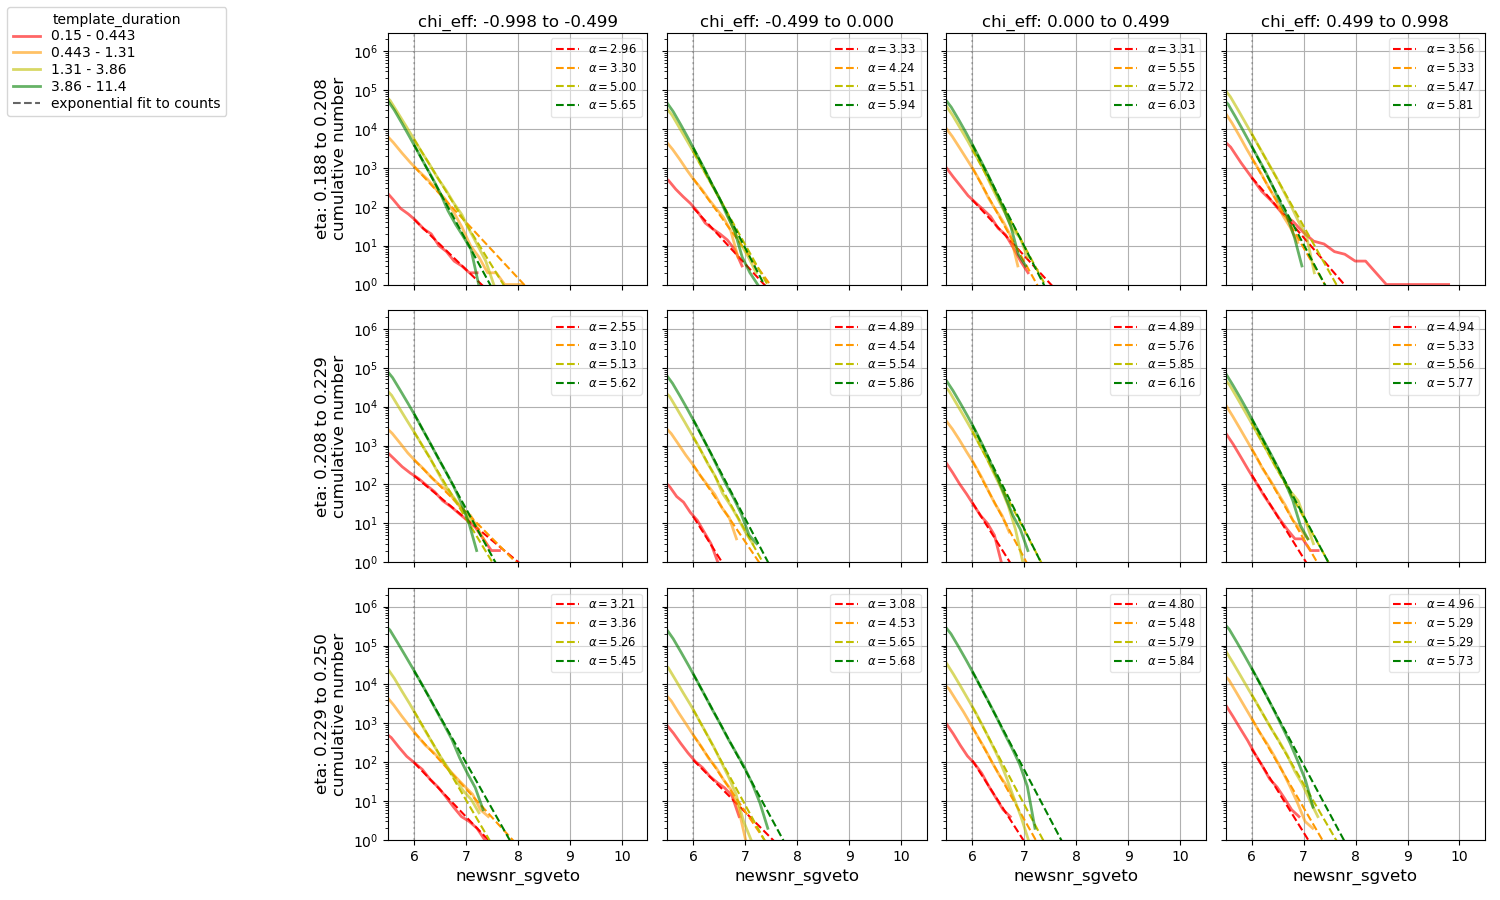
\includegraphics[width=0.49\textwidth]{images/pycbclive/H1-template_fits.png}
  \hspace{0.01\linewidth}
  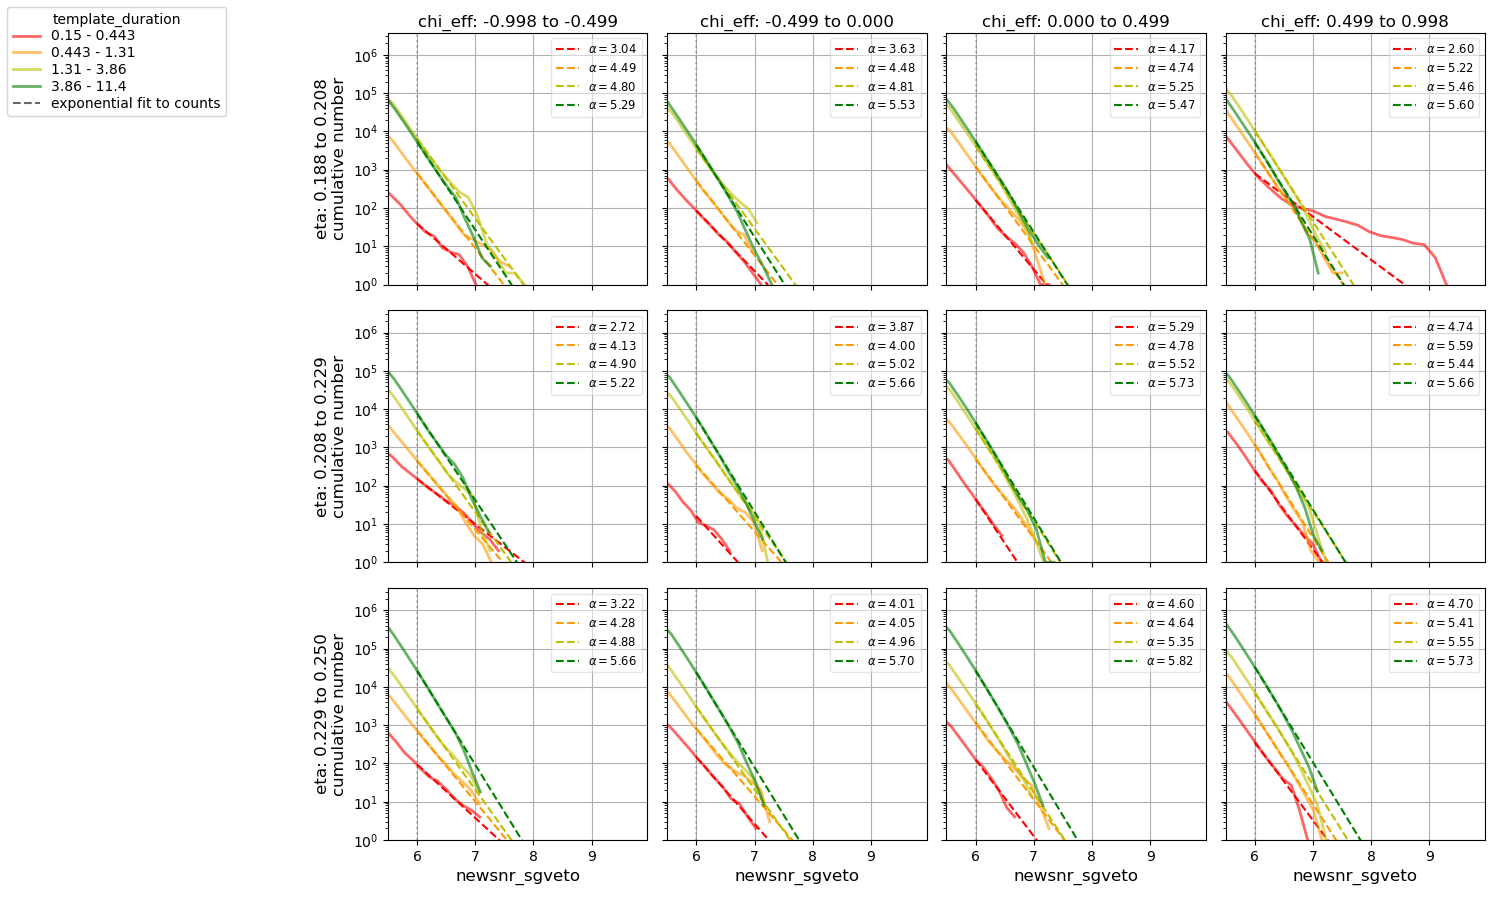
\includegraphics[width=0.49\linewidth]{images/pycbclive/L1-template_fits.png}
  \end{minipage}
  \caption{}
  \label{fig:pycbclive-fits}
\end{figure}
%
Figure~\ref{fig:pycbclive-fits} shows the associated fits made by the injection testing we did to measure the increase in sensitivity. These fits show good agreement to the exponential in the majority of the template bins except for the top-right for both H1 and L1 where there is an excess of high SNR triggers for these high-chieff, low eta and very short duration BBH templates.

\section{\label{Sensitivity Improvements}}

We measure improvement to the live search by performing injection set tests. The injection sets are made up of thousands of gravitational wave signals that are injected at a rate of approximately one every 100 seconds. We run two 'live' searches for gravitational waves, one with the old ranking statistic and one with the new ranking statistic which includes the additions of both PSD variation and template fitting.

The injection set used for this test is made up entirely of BBH signals to reduce the size of the template bank required~(CITE R\&P PAPER FOR O3), there is a limit to the amount of memory a user can request for this pseudo-live search and therefore we couldn't initially test these changes on the full pycbc live template bank. The template bank of 15436 templates covers the BBH signal parameter space and is described in this paper~(CITE O3 BBH PAPER?). 

The gravitational wave data used was a two week period of O3b where the first week was used to generate the template fits and the second week was used to test the fits. The injected gravitational wave data was created before the live searches were run and both searches were run on exactly the same data. While this search is emulating the live search it will very simply wait for new data before it moves forwards by eight seconds, if this data already exists (in the form of pregenerated data) then it will perform the processing as fast as it can. Therefore, a running the live search over a week of data does not take a whole week but it can take as little as 24 hours.

Once both searches have completed we can count the number of injections found by both searches. Theoretically the searches should both observe the exact same number of injections with almost identical triggers due to their nature but, computing isn't always perfect and therefore the searches observed slightly different amounts of time during the second week. This means that a simple count of injections found cannot be done, we need to isolate the injections seen in jointly observed time between the two searches.

This produced a list of injections seen by both searches in which we can directly compare the false alarm rate (or inverse false alarm rate, IFAR) of each injection to see if there has been an improvement. Each of these events is a real gravitational wave signal so we hope to see every single injection with a large IFAR value to indicate that the changes to the ranking statistic has improved the sensitivity of the search. Figure~\ref{fig:pycbclive-ifar-vs-ifar} displays the change in IFAR for each injection with the new statistic (colloquially referred to as 'fits') on the y-axis and the x-axis the old statistic IFAR values.
%
\begin{figure}
       \centering
    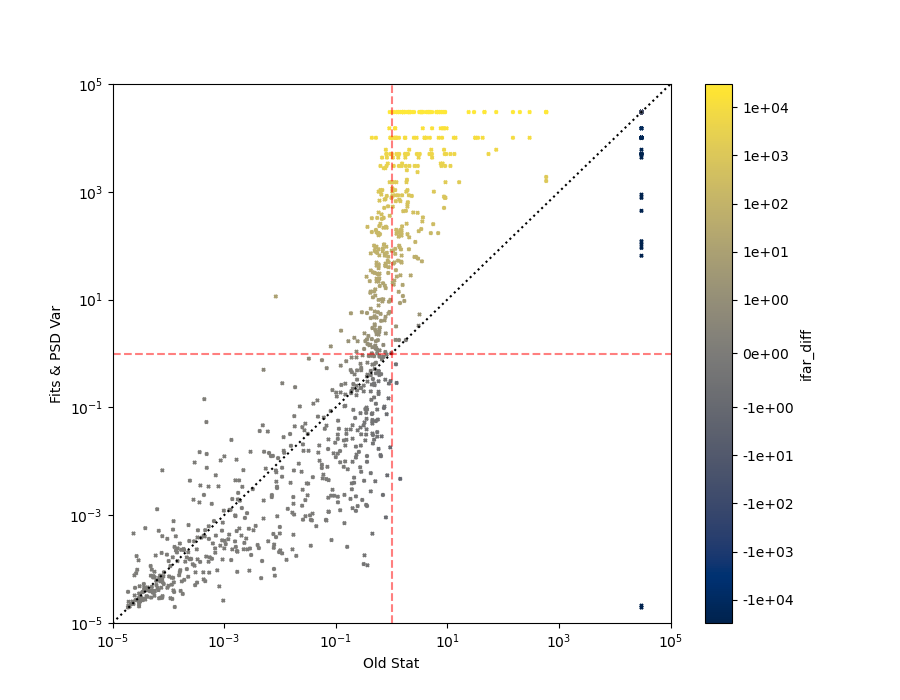
\includegraphics[width=1.2\textwidth]{images/pycbclive/fits_vs_old_colour.png}
    \caption{}
    \label{fig:pycbclive-ifar-vs-ifar}
\end{figure}
%
Within figure~\ref{fig:pycbclive-ifar-vs-ifar} we have plotted a vertical and horizontal dotted line at an IFAR of 1 year to indicate a commonly chosen IFAR limit of where an event would be considered 'real'. Therefore this figure can be split into four quadrants: top-left, injections originally missed below the IFAR threshold and now found above it; top-right, injections found in both searches; bottom-left, injections below the threshold by both searches; bottom-right, injections originally found above the IFAR threshold but missed with the new statistic. Another line has been plotted at y=x, injections above this line (in the top-left) have been found with a larger IFAR with the new statistics and injections below (in the bottom-right) have been found with a lower IFAR with the new statistic.

We have investigated all injections in the bottom-right quadrant and have found discrepancies in why these have been down-ranked which needs further investigation.


